\chapter{EXPERIMENTAL RESULTS AND DISCUSSION}

In this chapter, we will present a comprehensive analysis of the experimental results obtained from our implementation of the Spectral Transformation Lanczos algorithm for the symmetric definite generalized eigenvalue problem. We examine the algorithm performance on a test matrix, analyze the effects of ill-conditioning on convergence and accuracy, and compare the error bounds with what was predicted with direct methods.

\section{Software and Computational Environment}
The numerical experiments in this thesis are performed using the Python programming language together with the NumPy $2.0.2$ and SciPy $1.13.1$ libaries which makes function calls to optimized and efficient LAPACK and BLAS routines for linear algebra computations. These libraries ensure high-performance matrix operations and numerical stability. All computations are performed in \textbf{double precision} (64 bit floating point, \texttt{float64}) to maintain numerical accuracy and consistency.

For reproducibility, all code is written in Python $3.9.6$ and executed within a controlled environment using \texttt{virtualenv}. All numerical results have been validated by comparing different levels of precision where applicable and verifying consistency with analytical results when available. Code for the experiments is managed using version control with Git to ensure reproducibility and can be found in \href{https://github.com/AyobamiAdebesin/ayobami_thesis}{https://github.com/AyobamiAdebesin/ayobami\_thesis}

\section{Experimental Setup}
To evaluate the ST-Lanczos algorithm, we employ Algorithm~\ref{alg:problem_setup} \comm{You have parentheses around Algorithm and Section numbers.  That is standard for equations, but not for these things.  I would remove them and add a tilde to introduce space that won't break across lines.  I changed it here in the \LaTeX\ code.}to generate test matrices $A$ and $B$ with controlled eigenvalue distribution. For the purpose of this thesis, we will be testing with dense matrices The eigenvalues are divided into 3 distinct groups, each with a specified range (spread). For each of the three groups, a random set of eigenvalues was generated with a uniform distribution, ensuring that the eigenvalues are distributed evenly within their respective ranges.

\begin{itemize}
    \item[$\bullet$] Group $1$ contains $1000$ eigenvalues in the range $(10^{-3}, 10^{1})$
    \item[$\bullet$] Group $2$ contains $1000$ eigenvalues in the range $(10^1, 10^3)$
    \item[$\bullet$] Group $3$ contains $1000$ eigenvalues in the range $(10^3, 10^7)$
\end{itemize}

The three sets of eigenvalues are then concatenated into a single array $D \in \mathbb{R}^{3000 \times 3000}$, which is then used with a regularization hyperparameter $\delta = 10^{1}$, to generate $A$ and $B$ of size $3000 \times 3000$. Our shift is choosen to be $\sigma = 1.5 \times 10^3$. For this choice of $\delta$, the condition number of $A$ and $B$ are as follows:
\begin{equation*}
    \kappa(A) = 5.96 \times 10^{11}, \qquad \kappa(B) = 8.09 \times 10^2
\end{equation*}
As discussed in Section (\ref{sec:ProblemSetup}), $A$ and $B$ will be symmetric with $B$ being positive definite. \added{The matrix}\comm{there is a rule never to start a sentence with a mathematical symbol or equation} $B$ is factored using the SciPy \texttt{cholesky} method which calls LAPACK \textbf{\texttt{xPOTRF}}. We chose to use this since $B$ was designed to be strictly positive definite, which does not require us to use  pivoted Cholesky factorization. \added{If it were merely semidefinite, pivoting would be required.}  We run Algorithm \ref{alg:spectral_lanczos_algorithm} for $n=2000$ iterations for the spectral problem
\begin{equation}\label{eq:ShiftedInvertedProblem2}
	C_b^T (A-\sigma B)^{-1} C_b \mathbf{u} = \theta \mathbf{u}, \qquad \mathbf{u} \neq \mathbf{0}
\end{equation}
to compute the lanczos decomposition using various decompositions techniques for $A - \sigma B$ that was discussed in Section (\ref{sec:SpectralTransformationDescription}). We explored these techniques, discuss the expected residual bounds and discuss the results in the following sections.

\section{Residual and Error Analysis}
To evaluate the efficiency of the ST-Lanczos algorithm for the given problem, we define some metrics and also review some of the residual bounds theorems given in \cite{stewart2024spectraltransformationdensesymmetric}.

\begin{definition}[Lanczos Decomposition Residual]\label{def:DecompositionResidual}
	Let equation (\ref{eq:Lanczos_Decomposition}) be the decomposition obtained from the completion of Algorithm \ref{alg:spectral_lanczos_algorithm}. Then we define the relative residual as:\comm{I removed a blank line here.  You had started a paragraph right before the equation, which added extra space.}
	\begin{equation}\label{eq:DecompositionResidual}
		\text{Relative Decomposition Residual} = \frac{\|BQ_n - Q_nT_n - \delta_{n}\mathbf{q}_{n+1}\mathbf{e}_n^T\|}{\|B\|},
	\end{equation}
	where $B = C_b^T (A-\sigma B)^{-1} C_b $.
\end{definition}
This residual measures how well the Lanczos algorithm has approximated the eigenvalues of $B$ through the tridiagonal matrix $T_n$.

\begin{definition}[Generalized Relative Residual]\label{def:GeneralizedRelativeResidual}
	Let $(\alpha_i, \beta_i)$ be the generalized eigenvalues of $A$ and $B$, and $\mathbf{v}_i \neq \mathbf{0}$ be the corresponding computed eigenvector obtained from computing the eigenvalues of $T_n$, such that $\mathbf{r}_i = (\beta_i A - \alpha_i B)\mathbf{v}_i$. Then we define the relative residual for each $i = 1, 2, \ldots n$ as:
	\begin{equation}\label{eq:GeneralizedResidual}
		\|\tilde{\mathbf{r}}_i\| = \frac{\| (\beta_i A - \alpha_i B)\mathbf{v}_i \| }{(\lvert \beta_i \rvert \|A\| - \lvert \alpha_i \rvert \|B\|)\|\mathbf{v}_i\| }
	\end{equation}
\end{definition}

\begin{definition}[Spectral Transformed Residual]\label{def:SpectralTransformedResidual}
	Let $(\theta_i, \mathbf{u}_i)$ be the Ritz-pair obtained from computing the eigenvalues and eigenvectors of $T_n$. Then we define the relative residual for each $i = 1, 2, \ldots n$ as:\comm{another blank line removed}
	\begin{equation}\label{eq:STResidual}
		\text{ST Relative Residual} = \frac{\| C_b^T(A - \sigma B)^{-1}C_b \mathbf{u}_i - \lvert \theta_i \rvert \mathbf{u}_i \| }{( C_b^T(A - \sigma B)^{-1}C_b + \lvert \theta_i \rvert)\|\mathbf{u}_i\| }
	\end{equation}
        \comm{in the numerator, it should be just $\theta_i$, not $|\theta_i|$.}
\end{definition}

\begin{definition}[Best Residuals]\label{def:BestResidual}
	Let $(\alpha_i, \beta_i)$ be the computed generalized eigenvalues of $A$ and $B$. We define the ``best relative residuals'' for $(\alpha_i, \beta_i)$ as
	\begin{equation}\label{eq:BestResiduals}
		\|\tilde{\mathbf{r}}_i\| = \frac{\sigma_n(\beta_i A - \alpha_i B)}{(\lvert \beta_i \rvert \|A\| - \lvert \alpha_i \rvert \|B\|)}
	\end{equation}
where $\sigma_n$ is the smallest singular value of the matrix pencil $(\beta_i A - \alpha_i B)$.
\end{definition}
This residual assess the quality of the computed eigenvalues independently of the eigenvectors. The smallest singular value is used to determine the ``\textbf{best achievable residual}'' for the eigenvalue pair $(\alpha_i, \beta_i)$, even with an idealized eigenvector.

We reference the following theorem(s) and lemma(s) from \cite{stewart2024spectraltransformationdensesymmetric}, which gives the residual bounds for computed eigenvalues and eigenvectors using the direct method employed in the paper. It should be noted that these bounds are not dependent on the exact algorithm used in computing the eigenvalues and eigenvectors. We will be using these bounds to evaluate the efficiency and stability of the ST-Lanczos algorithm used in this thesis and validate our computed residuals with these bounds.

\begin{theorem}[Residual Bounds for Eigenvalues]\label{thrm:ResidualBoundsEigenvalues}
	Let $C_a, C_b, X, \eta,$ and $\theta_i$ be computed quantities using a direct method described in \cite{stewart2024spectraltransformationdensesymmetric}. Let $E, F, F_1, e_n,$ and $f_n$ be as in Theorem 3.1. Suppose that $(A + E) - \sigma(B + F)$ is invertible. Without loss of generality, assume that the computed eigenvalues $\theta_i$ are in nondecreasing order and let $\hat{\theta}_i$ and $\hat{u}_i$ for $i = 1, 2, \dots, r$ be eigenvalues and eigenvectors of
	\[
	\hat{W} = (C_b + F_1)^{T} (A + E - \sigma(B + F))^{-1}(C_b + F_1)
	\]
	with the $\hat{\theta}_i$ also in nondecreasing order. Assume that $(C_b + F_1) \hat{u}_i \neq 0$ and define
	\[
	\hat{v}_i = (A + E - \sigma(B + F))^{-1} (C_b + F_1) \hat{u}_i \neq 0.
	\]
	 Then
	\begin{align*}
		&\|(\theta_i (A + E) - (1 + \sigma \theta_i) (B + F)) \hat{v}_i \|_2
		\leq \\
		& u (e_n + f_n)(1 + | \sigma_0 |) \eta^2 \| X \|_2^2 \left( | \theta_i | \| A + E \|_2 + | 1 + \sigma \theta_i | \| B + F \|_2 \right) \| \hat{v}_i \|_2 + O(u^2).
	\end{align*}
where $\hat{v}_i$ is the exact eigenvector of the perturbed problem, and not a computed eigenvector using the lanczos procedure.
\end{theorem}
\comm{You are missing bold vectors here and in the following theorems.  You are going to need to say more about $\eta \|X\|_2$ and its definition, but it will be easier if you put the main spectral transformation lemma in Chapter~1 so you can refer back to it.  Not having that Lemma is going to make it hard to finish this chapter.}
The implication of this theorem is that the residuals of the computed eigenvalues depends on $\eta^2 \| X \|_2^2$, a scaled shift $\sigma_0$ and the alignment of $\sigma$ with the eigenvalues. The quantities $\eta^2 \| X \|_2^2$ and  $\sigma_0$  are quantities from the original paper and are not of much importance in this context, but what is important for us to note here is that choosing the shift $\sigma$ to avoid \added{extreme} proximity to eigenvalues \rep{can be shown to give reasonable bounds on $\eta \|X\|_2$.}{will minimize residuals.} That is, for eigenvalues $\lambda_i = (1 + \sigma \theta_i)/ \theta_i$, the residuals will remain small if $\sigma$ is not too close to $\lambda_i$.

\begin{lemma}[Residual Bounds for Computed Eigenvectors]\label{lemma:ResidualBoundsEigenvectors}
		Let $C_a, C_b, X, \theta_i \neq 0,$ and $U$ be computed quantities from Algorithm 1. Let $\eta$ and $\gamma$ be as in (2.5) and (2.8). Let the errors associated with the algorithm be as in Theorem 3.1. If $v_i$ is computed from $C_a^T v_i = D_a X u_i$ using a backward stable algorithm for the solution of the system and standard matrix-vector multiplication for forming the right-hand side, then
		\[
		\| \left( \theta_i A - (1 + \sigma \theta_i) B \right) v_i \|_2 \leq u c_n + O(u) \Bigg[ \eta \| X \|_2 \\
		+ \left( 1 + \frac{1}{| \eta^2 \theta_i |} + \max(\gamma, 1) \right) \eta^2 \| X \|_2^2 \Bigg] \| B \|_2 \| v_i \|_2.\]
\end{lemma}

\begin{theorem}\label{thrm:ResidualBounds}
	Assume that $\sigma\neq 0$ and $\lambda_i\neq 0$.  Under the assumptions of Lemma (\ref{lemma:ResidualBoundsEigenvectors}), we have
	\begin{multline*}
		\left\| \big(\theta_i A - (1+\sigma \theta_i) B\big) \vec{v}_i \right\|_2
		\leq \\
		|1+\sigma \theta_i| \cdot |1-\sigma/\lambda_i| \Bigg[
		uc_n +O(u)\Bigg( \eta\|X\|_2 \\
		+ \left(1 + \max(\gamma, 1)
		\left(1+ \left| 1 - \frac{\lambda_i}{\sigma}\right|\right)\right)
		\eta^2\|X\|_2^2 \Bigg) \Bigg] \|B\|_2 \|\vec{v}_i\|_2,
	\end{multline*}
	and
	\begin{multline*}
		\left\| \big(\theta_i A - (1+\sigma \theta_i) B\big) \vec{v}_i \right\|_2
		\leq \\
		|\theta_i| \cdot |1-\lambda_i/\sigma| \cdot |\sigma_0| \Bigg[
		uc_n +O(u)\Bigg( \eta\|X\|_2 \\
		+ \left(1 + \max(\gamma, 1) \left(1+ \left| 1
		- \frac{\lambda_i}{\sigma}\right|\right)\right)
		\eta^2\|X\|_2^2 \Bigg) \Bigg] \|A\|_2 \|\vec{v}_i\|_2,
	\end{multline*}
\end{theorem}
\comm{In these, in the preamble I define \textbackslash vec to give bold vectors.  I've added that, so you can merge it in and won't have little arrows above vectors.}
Lemma( \ref{thrm:ResidualBounds}) establishes a foundational bound for the eigenvector residual, emphasizing the role of $\eta = \|A - \sigma B\|_2^{1/2}/\|B\|_2^{1/2} $, which quantifies the stability of solving systems involving $A-\sigma B$, in making sure that the residuals for the computed eigenvectors are bounded. Small residuals require $\eta \|X\|_2$ (where $X = C_a^{-1}C_b$) to remain moderate, which is achievable through stable factorizations like pivoted Cholesky for $B$ and rook pivoting $LDL^T$ for $A-\sigma B$.

On the other hand, Theorem (\ref{thrm:ResidualBounds}) which builds on Lemma (\ref{lemma:ResidualBoundsEigenvectors}), refines this into two interpretations. The first interpretation is that residuals scale with $\lvert 1 - \sigma/ \lambda_i \rvert$, ensuring accuracy when $\sigma$ aligns closely with $\lambda_i$. The second interpretation is that choosing large shifts will cause the residuals to grow unless $\lambda_i$ is near $\sigma$. This behavior will tend to occur even if the best residuals are computed with (\ref{eq:BestResiduals}).

So the key takeaway useful for this thesis is, in order to ensure small residuals and stability, the shift $\sigma$ should not be too close to any generalized eigenvalue and should not be too large in magnitude. A moderate shift will guarantee small residuals for eigenvalues not much larger than $\sigma$ but a large shift will result in having small residuals only for eigenvalues near $\sigma$.

\section{$LU$ decomposition}

The $LU$ decomposition of $A - \sigma B$ is performed using the \texttt{linalg.lu\_factor} function in SciPy, which employs partial pivoting. With a moderately large shift $\sigma = 1.5 \times 10^3$ not close to a generalized eigenvalue and for $n = 2000$ iterations, the Krylov solution subspace has a dimension of $2000$, and the ST Lanczos algorithm achieves a decomposition residual, computed with (\ref{eq:DecompositionResidual}), to the order of $10^{-11}$, despite a full reorthogonalization. This reduction in accuracy is attributed to pivot-limited accuracy. Using a tolerance of $10^{-10}$ for the Ritz pair residuals computed with (\ref{eq:STResidual}), approximately $76\%$ of the Ritz pairs converge to within an accuracy of order $10^{-14}$.

On the other hand, the generalized residuals for these converged Ritz pairs are close to the order of machine precision $u=10^{-15}$ for generalized eigenvalues not much larger than the shift. As shown in Fig \ref{fig:LUResidualsModShift}, the residuals are small for eigenvalues that are close to or smaller in magnitude than the shift and gradually tends to increase for larger eigenvalues, consistent with the error bounds stated in Theorem (\ref{thrm:ResidualBounds}) for a direct method, indicating that the residuals scale with $\lvert 1-\sigma/\lambda_i \rvert$. This scale factor appears in one of the error bounds in Theorem (\ref{thrm:ResidualBounds}). The third plot\comm{Not in this draft.  I'm wondering if it was left out by accident or if you are still working on it and just put this text in before adding the graph.} shows the best possible relative residuals for some choice of $\mathbf{v}_i$. This is the best residuals described in (\ref{def:BestResidual}). This shows that every computed eigenvalue can result in a small residual, validating the bound given in Theorem (\ref{thrm:ResidualBoundsEigenvalues}).

\begin{figure}
	\centering
	\caption{Residuals plot for a well-conditioned problem with moderate shift $\sigma=1.5 \times 10^3$}
	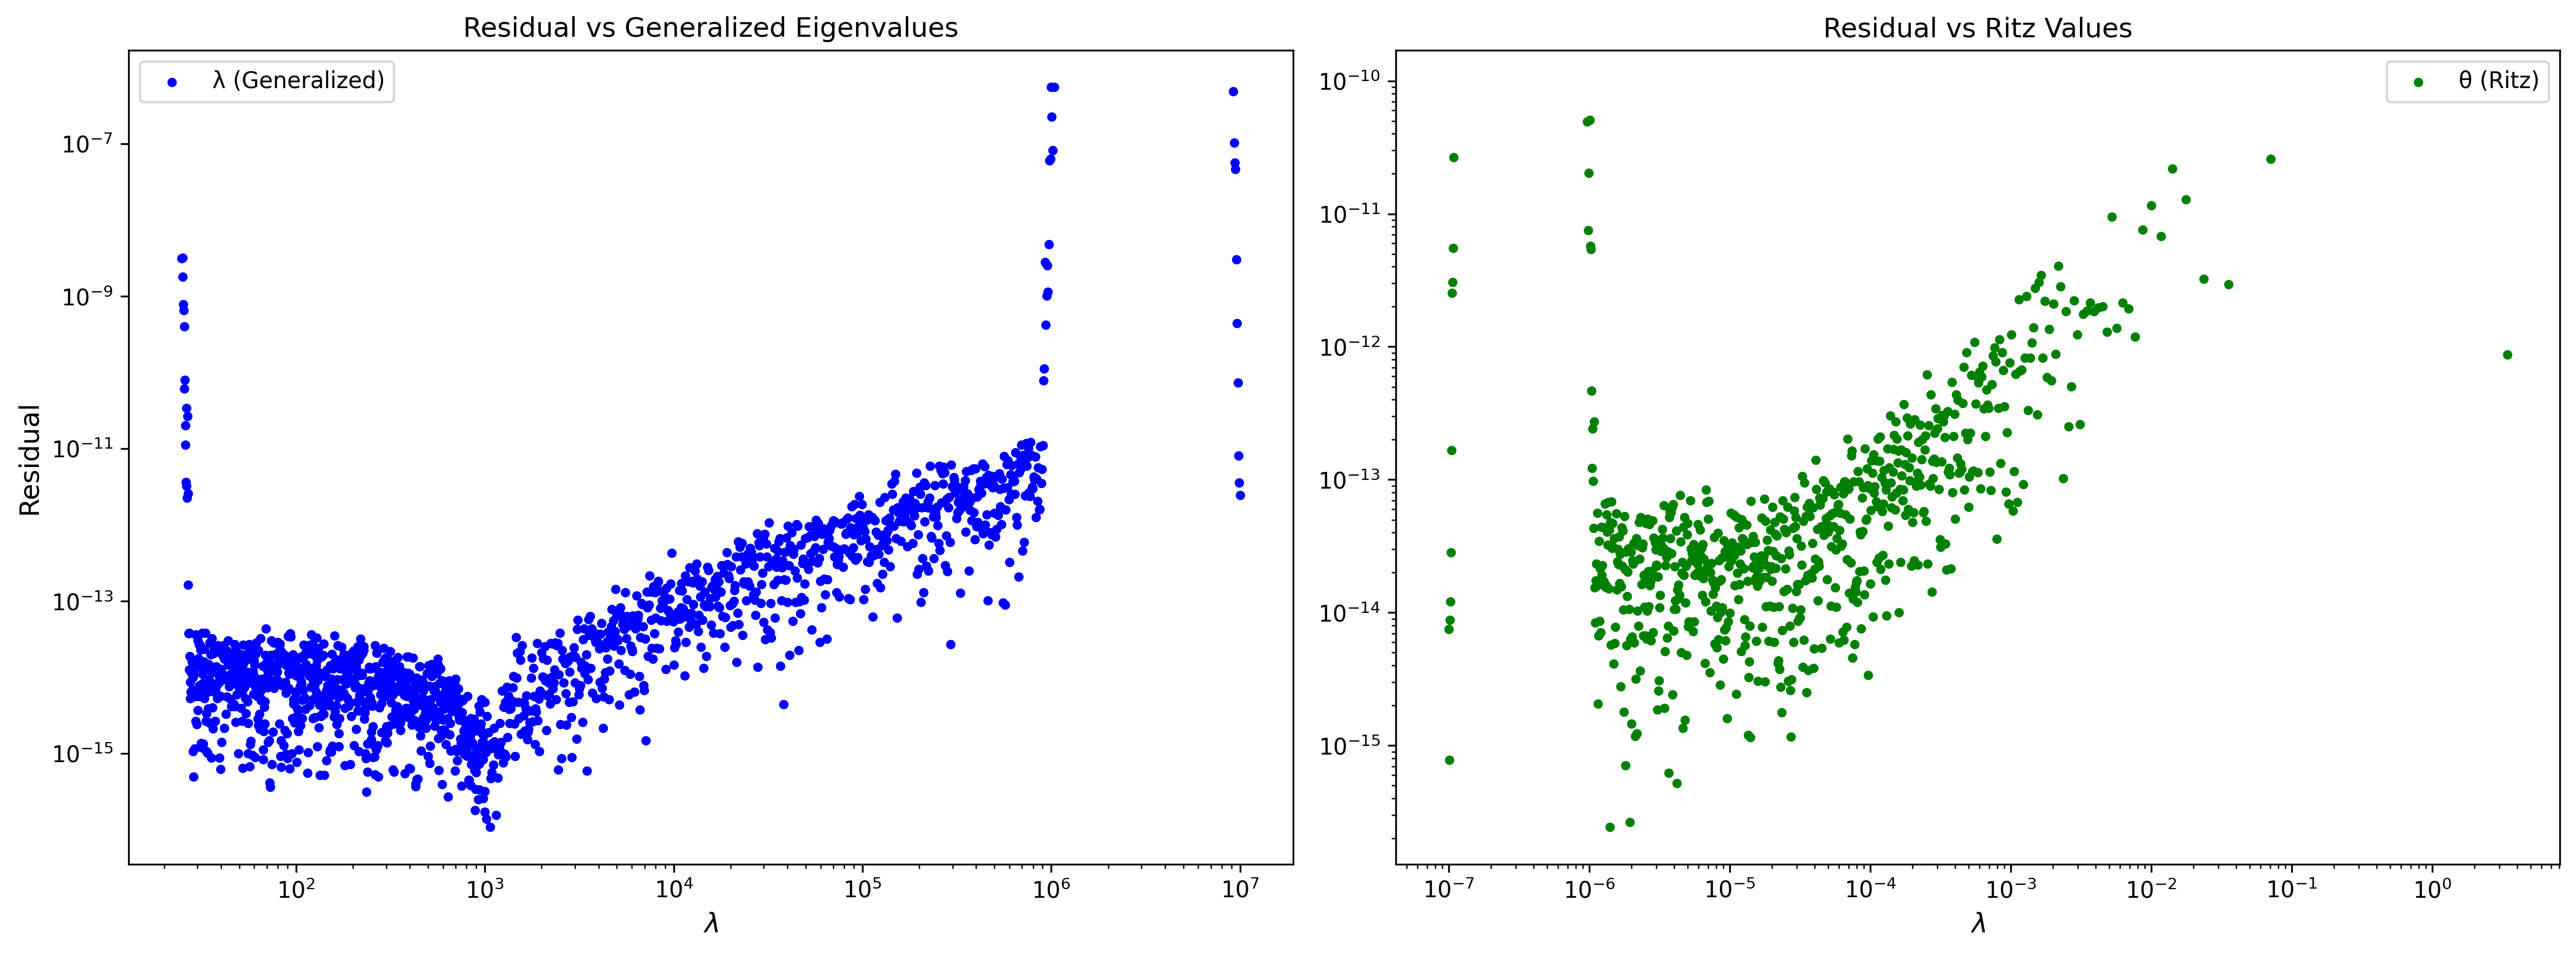
\includegraphics[height=2.5in]{./Plots/LU/residuals_plot_well_mod.png}
	
	\label{fig:LUResidualsModShift}
\end{figure}

For a shift that is large in magnitude, we consider $\sigma = 1.5 \times 10^5$. Running the algorithm with the same parameters as described for the moderate shift, it is observed that the computed eigenvalues and eigenvectors delivers small residuals for eigenvalues that are not too much larger or smaller in magnitude than $\sigma$. The left plot of Figure (\ref{fig:LUResidualsLargeShift}) shows that for eigenvalues that are orders of magnitude smaller than the shift, the residuals are way smaller. Although, this might not be evident in the plot, but the fact that they are smaller.
%To examine the effect of conditioning, $\delta$ was increased to $\delta=10^2$ so that $\kappa(A) = 1.5 \times 10^{10}$ and $\kappa(B) = 81.8$. For this \textit{well-conditioned} problem, the Lanczos decomposition residual decreases to the order of $10^{-11}$, indicating that the accuracy of the Lanczos decomposition is influenced by the problem's conditioning. Additionally, for the same tolerance, $68\%$ of Ritz pairs converged, with a decrease in residuals to the order of $10^{-15}$ while a similar trend can be seen for the generalized eigenvalues as shown in Figure \ref{fig:LUResidualsWell}.


\begin{figure}
	\centering
	\caption{Residuals plot for a well-conditioned problem with large shift $\sigma=1.5 \times 10^5$}
	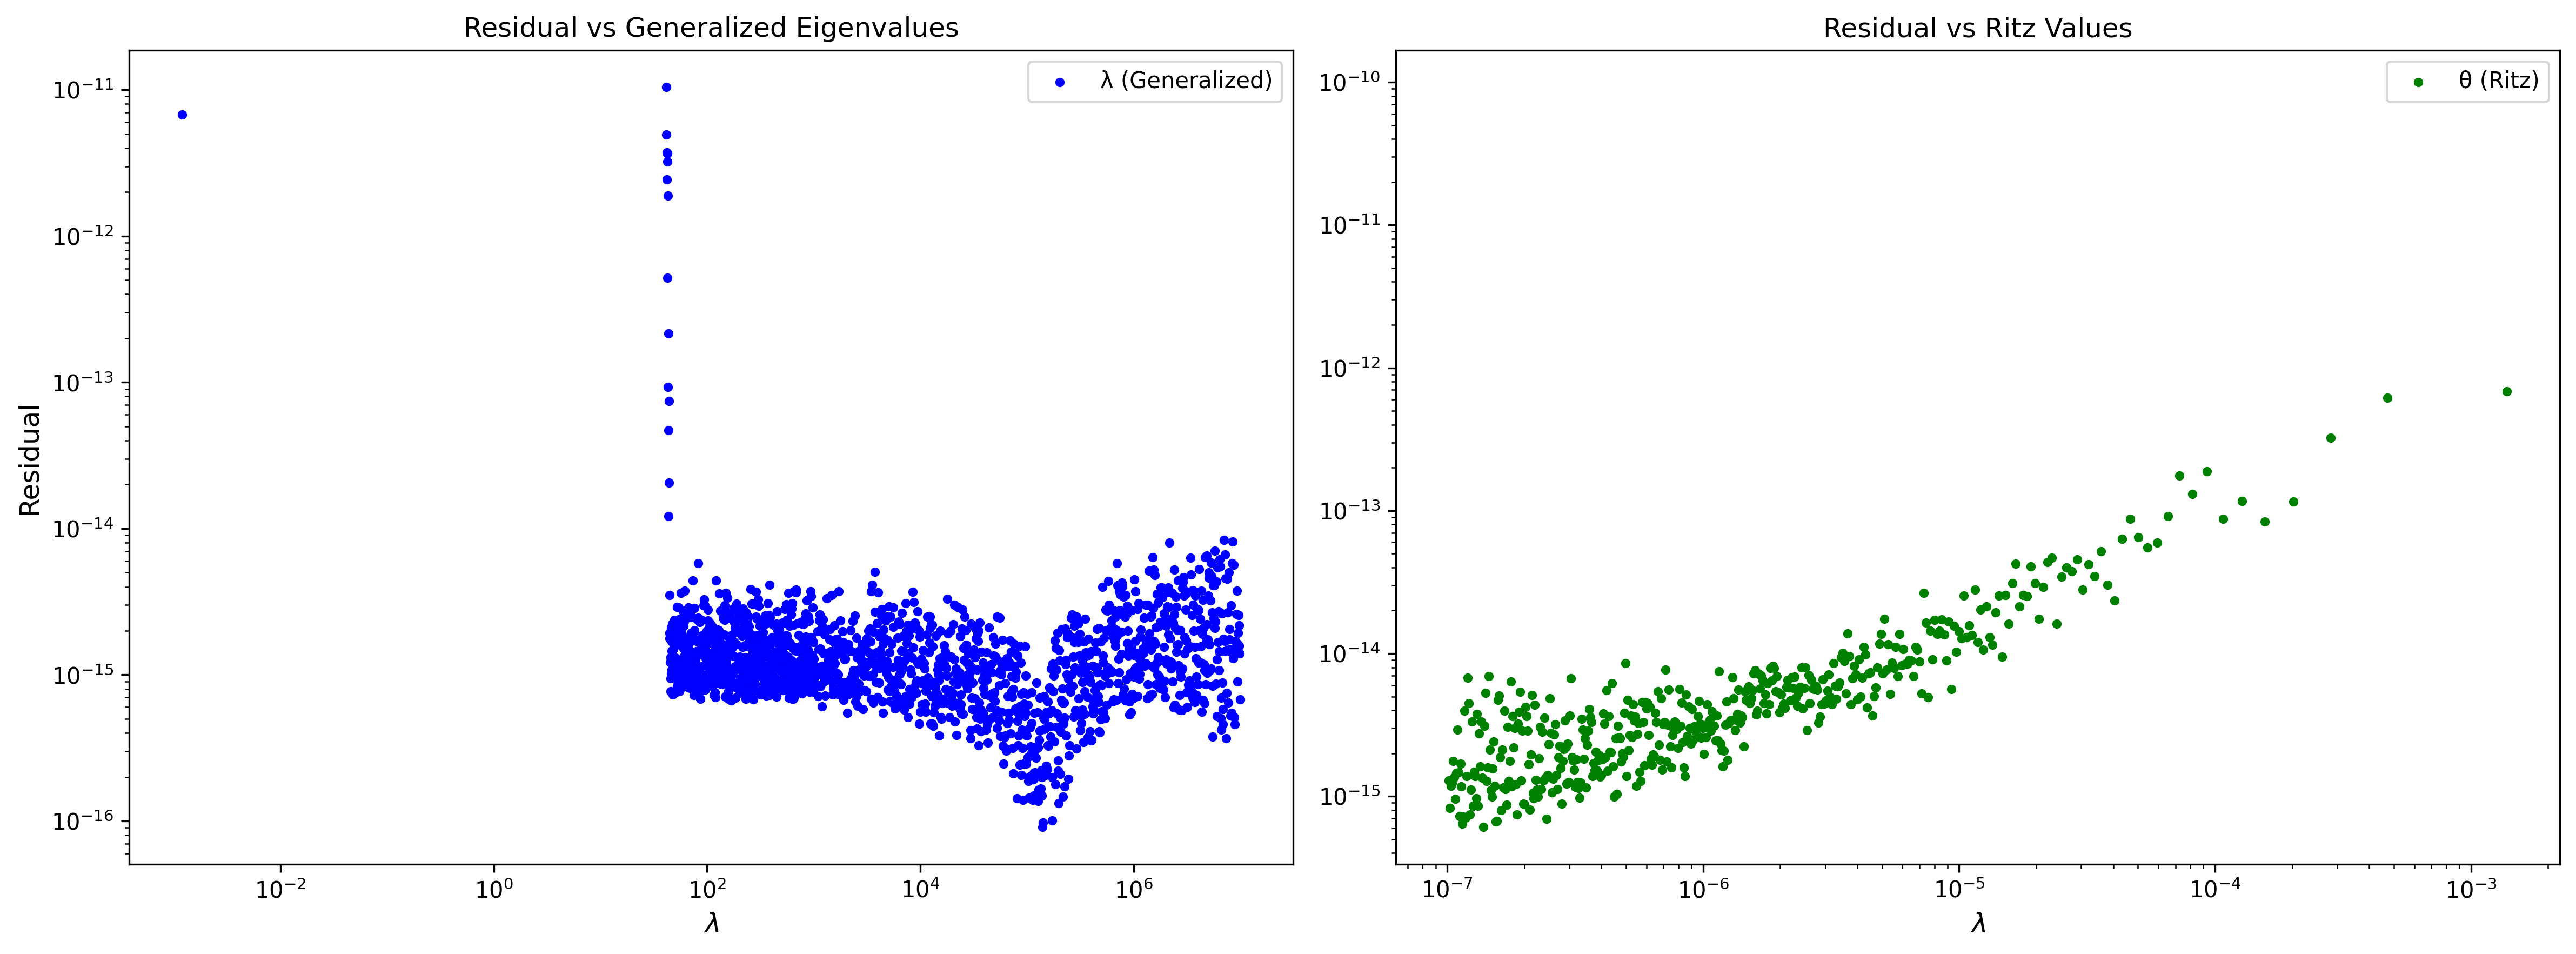
\includegraphics[height=2.5in]{./Plots/LU/residuals_plot_well_large.png}
	
	\label{fig:LUResidualsLargeShift}
\end{figure}



\section{Eigenvalue Decomposition}
Another decomposition technique we employed is the symmetric eigenvalue decomposition of $A-\sigma B$ given by
\begin{equation}
    A-\sigma B = WDW^T,
\end{equation}
so that the spectral transformed problem is given by
\begin{equation}\label{3.4}
	C_b^T W^{-T}D^{-1}W^{-1} C_b \mathbf{u} = \theta \mathbf{u}, \qquad \mathbf{u} \neq \mathbf{0}
\end{equation}
This decomposition, done using \texttt{linalg.eigh} function in SciPy, uses the LAPACK \texttt{dsyevd} routine for real symmetric matrices, which in turn uses divide-and-conquer algorithms for efficiency. The Lanczos decomposition residual was observed to be of the order $10^{-23}$, indicating a highly accurate decomposition.
%On the left plot, the residuals remain on the order of machine precision $10^{-17}$ for most eigenvalues. Similarly, on the right of the plot, the Ritz residuals are minimized near $\theta = 0$ with values on the order of machine precision and gradually increasing for larger Ritz values. To assess the effect of ill-conditioning, $\delta$ was reduced to $\delta = 10^{-5}$, so that $\kappa(A) = 8.2 \times 10^9$ and $\kappa(B) = 5.4 \times 10^8$. It was observed that this ill-conditioning did not affect the computed residuals with.\\
%Overall, the extremely low decomposition residual confirms the robustness of using a decomposition that preserves symmetry, while the observed trends in residuals highlight the sensitivity of numerical accuracy to the spectrum of the problem.

%%% Local Variables:
%%% mode: LaTeX
%%% TeX-master: "../main"
%%% End:
